\documentclass{article}
\usepackage[T1]{fontenc}
\usepackage{lmodern}
\usepackage{graphicx}
\usepackage{amsmath,amssymb}
\usepackage[a4paper,margin=2cm]{geometry}
\usepackage[absolute,overlay]{textpos}
\setlength{\TPHorizModule}{1mm}
\setlength{\TPVertModule}{1mm}
\usepackage[indonesian]{babel}
\usepackage{hyperref}
\setlength{\emergencystretch}{2em}
% unit: Halaman 34

\begin{document}

% === Halaman 34 (llm) ===

Filtering dengan penerapan Wireshark dapat menampilkan plainteks berupa username dan password\vspace{10mm}

\vspace{115.83mm}

Sumber gambar: https://www.researchgate.net/figure/Wireshark-Filtering-Showing-Clear-Text-of-user-Name-and-Password\_fig3\_326419957

% deskripsi: Screenshot aplikasi Wireshark yang menunjukkan proses analisis paket HTTP POST, memperlihatkan data form yang tidak terenkripsi berisi username 'Ibrahim\_Diyeb' dan password 'yemen\_123'.
% bbox normalisasi: [0.1050, 0.3300, 0.8450, 0.7200]
\begin{textblock*}{155.40mm}(22.05mm,98.01mm)
\noindent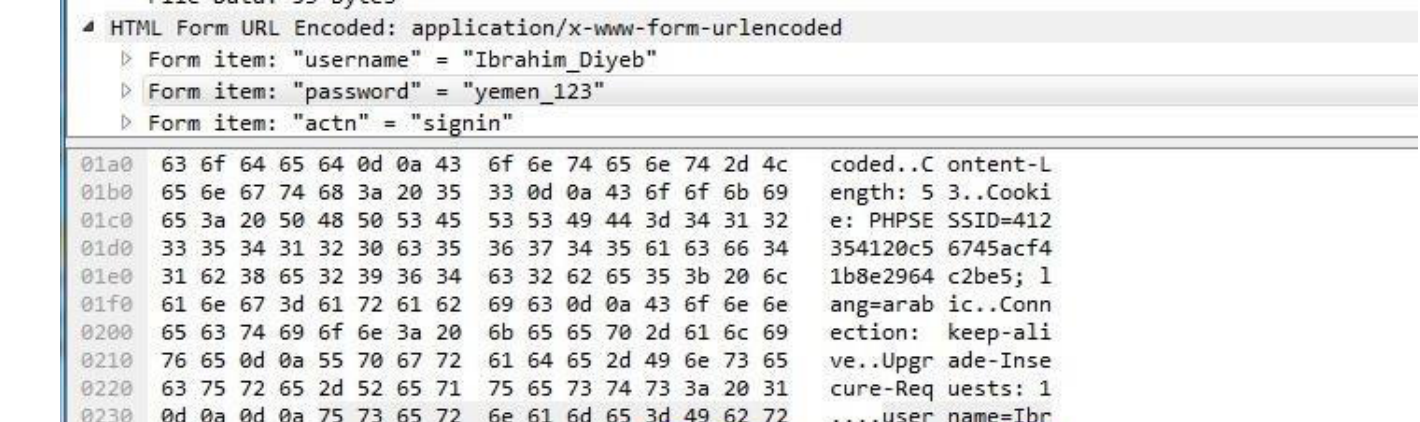
\includegraphics[width=155.40mm,height=115.83mm]{../../images/llm/page_034_img_01.png}%
\end{textblock*}

\end{document}
